\begin{recipe}
[ %
        preparationtime = {\SI{20}{\hour}},
        bakingtime={\SI{1}{\hour}},
        bakingtemperature={\protect\bakingtemperature{topbottomheat=\SI{280}{\celsius}}},
        portion = {\portion[Loaf]{1}},
        source = {Hiramas}
    ]{Hirabread}
	    
	    \begin{figure}[p]
	        \centering
	        \makebox[\textwidth][c]{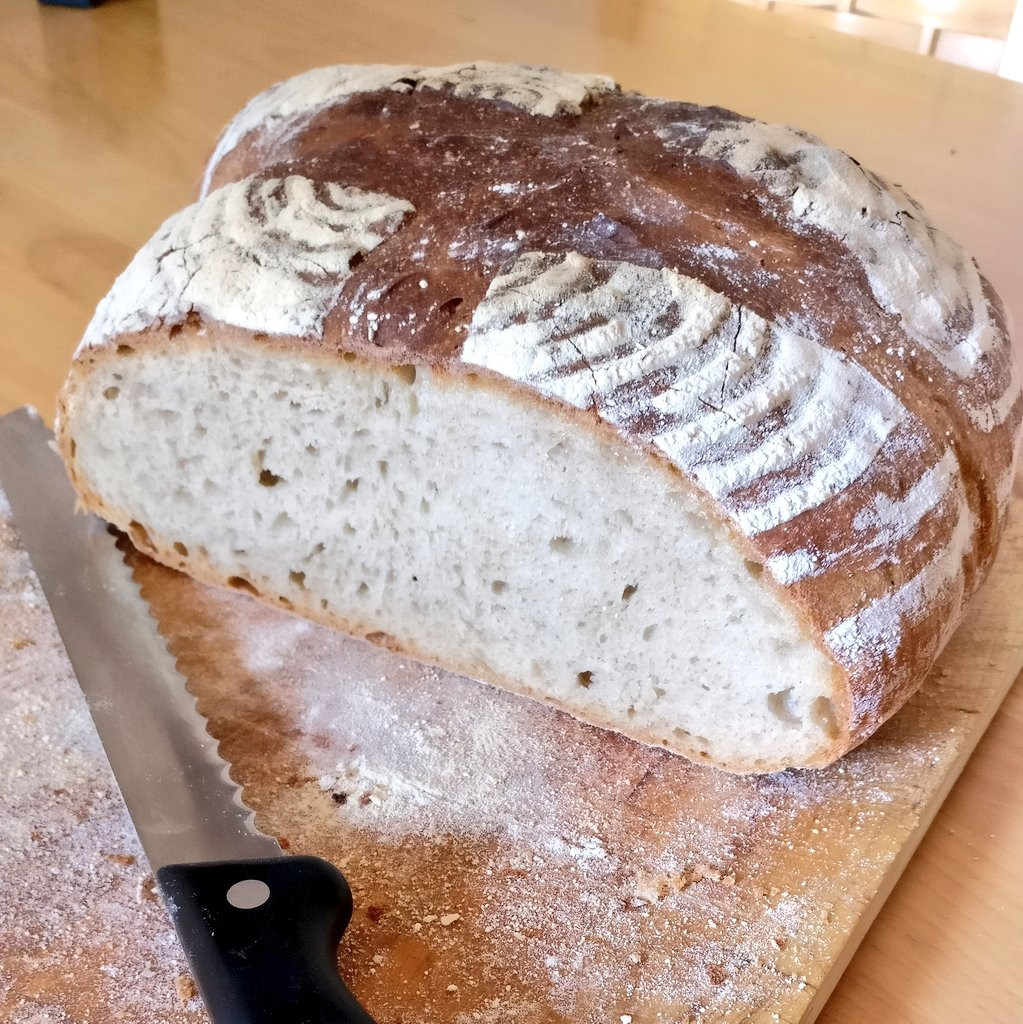
\includegraphics[height=\textheight]{hirabread/EV0I-6cUcAkaNUL.jpg}}
	    \end{figure}
	    
		\ingredients[14]{
		    \multicolumn{2}{c}{\textbf{Rye preferment}} \\
		    \SI{120}{\gram} & Rye flour 1150 \\
		    \SI{100}{\gram} & Water \\
		    \SI{8}{\gram} & Starter \\
		    & \\
		    \multicolumn{2}{c}{\textbf{Wheat preferment}} \\
		    \SI{75}{\gram} & Wheat flour 550 \\
            \SI{75}{\gram} & Water \\
            \SI{0.1}{\gram} & Fresh baker's yeast \\
            & \\
            \multicolumn{2}{c}{\textbf{Main dough}} \\
            \SI{375}{\gram} & Wheat flour 1050 \\
            \SI{125}{\gram} & Wheat flour 550 \\
            \SI{13}{\gram} & Salt \\
            \SI{6}{\gram} & Fresh baker's yeast \\
            \SI{300}{\gram} & Water 
		}
		
		\preparation {
		    \step Mix the rye dough and let ferment for \SI{18}{\hour} at a falling temperature, from \SIrange{30}{20}{\celsius}.
		    \step Mix the wheat dough and let ferment for \SI{18}{\hour} at \SI{20}{\celsius}.
		    \step Knead the dough and rest for \SI{45}{\minute} at \SI{24}{\celsius}.
		    \step Shape the dough, let rest for \SI{50}{\minute} at \SI{24}{\celsius}.
		    \step Bake the dough, with seam down, and scored with a cross, starting at \SI{280}{\celsius}, falling to \SI{200}{\celsius} for \SI{60}{\minute}.
		}
\end{recipe}